\documentclass[11pt,twocolumn]{article}

% ------------------------------------------------------------
% Page layout
% ------------------------------------------------------------
\usepackage[letterpaper,margin=0.75in]{geometry}
\usepackage{microtype}
\usepackage{parskip}
\setlength{\columnsep}{0.25in}

% ------------------------------------------------------------
% Core math
% Load amsmath/mathtools before unicode-math.
% ------------------------------------------------------------
\usepackage{amsmath}
\usepackage{mathtools}

% ------------------------------------------------------------
% Fonts: LuaLaTeX or XeLaTeX
% ------------------------------------------------------------
\usepackage{fontspec}
\usepackage{unicode-math}

\setmainfont{DejaVu Serif}
\setsansfont{DejaVu Sans}
\setmonofont{DejaVu Sans Mono}
\setmathfont{Latin Modern Math}

% Do NOT load amssymb, amsfonts, or bm with unicode-math.
% amssymb/amfonts can conflict with symbols such as \eth.
% bm can break Greek bold symbols under unicode-math.

% ------------------------------------------------------------
% Extra math utilities
% ------------------------------------------------------------
\usepackage{tensor}
\usepackage{cancel}

% ------------------------------------------------------------
% Tables
% ------------------------------------------------------------
\usepackage{booktabs}
\usepackage{array}
\usepackage{tabularx}
\usepackage{multirow}
\usepackage{siunitx}

\sisetup{
  detect-all,
  per-mode=symbol,
  exponent-product=\cdot
}

% ------------------------------------------------------------
% Figures, SVG, PGF/TikZ plots
% ------------------------------------------------------------
\usepackage{graphicx}
\usepackage{svg}
\usepackage{tikz}
\usepackage{pgfplots}
\usepackage{stfloats}

\pgfplotsset{compat=1.18}

\usetikzlibrary{
  arrows.meta,
  calc,
  positioning,
  decorations.pathmorphing,
  matrix
}

% ------------------------------------------------------------
% Captions and references
% ------------------------------------------------------------
\usepackage{caption}
\usepackage{subcaption}
\usepackage[hidelinks]{hyperref}
\usepackage[nameinlink,noabbrev]{cleveref}

% ------------------------------------------------------------
% Common math macros
% ------------------------------------------------------------

% Sets and spaces
\newcommand{\R}{\mathbb{R}}
\newcommand{\C}{\mathbb{C}}
\newcommand{\N}{\mathbb{N}}
\newcommand{\Z}{\mathbb{Z}}
\newcommand{\Q}{\mathbb{Q}}

\newcommand{\Ltwo}{L^2}
\newcommand{\Lp}[1]{L^{#1}}
\newcommand{\Hsob}[1]{H^{#1}}
\newcommand{\Cinfty}{C^\infty}

% Scalars, vectors, matrices, tensors
\newcommand{\scal}[1]{#1}
\newcommand{\vct}[1]{\symbfit{#1}}   % bold italic vector, works for Greek
\newcommand{\mat}[1]{\symbf{#1}}     % bold upright matrix
\newcommand{\ten}[1]{\symbfsf{#1}}   % bold sans-serif tensor

% Unit vectors
\newcommand{\ihat}{\hat{\vct{i}}}
\newcommand{\jhat}{\hat{\vct{j}}}
\newcommand{\khat}{\hat{\vct{k}}}

% Transpose, inverse, trace, determinant
\newcommand{\T}{^{\mathsf{T}}}
\newcommand{\inv}{^{-1}}
\newcommand{\tr}{\operatorname{tr}}
\newcommand{\diag}{\operatorname{diag}}
\newcommand{\rank}{\operatorname{rank}}
\newcommand{\nullspace}{\operatorname{null}}
\newcommand{\range}{\operatorname{range}}
\newcommand{\determinant}{\operatorname{det}}

% Norms, inner products
\newcommand{\norm}[1]{\left\lVert #1 \right\rVert}
\newcommand{\abs}[1]{\left\lvert #1 \right\rvert}
\newcommand{\inner}[2]{\left\langle #1, #2 \right\rangle}

% Differential operators
\newcommand{\dd}{\,\mathrm{d}}
\newcommand{\pd}{\partial}
\newcommand{\grad}{\nabla}
\newcommand{\divg}{\nabla \cdot}
\newcommand{\curlop}{\nabla \times}
\newcommand{\rot}{\nabla \times}
\newcommand{\laplace}{\Delta}

% Derivatives
\newcommand{\dv}[2]{\frac{\mathrm{d} #1}{\mathrm{d} #2}}
\newcommand{\dvtwo}[2]{\frac{\mathrm{d}^2 #1}{\mathrm{d} #2^2}}
\newcommand{\pdv}[2]{\frac{\partial #1}{\partial #2}}
\newcommand{\pdvtwo}[2]{\frac{\partial^2 #1}{\partial #2^2}}

% Matrix exponential
\newcommand{\expm}{\operatorname{expm}}

% Complex / imaginary numbers
\newcommand{\ii}{\mathrm{i}}
\newcommand{\Real}{\operatorname{Re}}
\newcommand{\Imag}{\operatorname{Im}}

% Fourier transform
\newcommand{\FT}{\mathcal{F}}
\newcommand{\IFT}{\mathcal{F}^{-1}}
\newcommand{\fourier}[1]{\widehat{#1}}

% Probability and statistics
\newcommand{\E}{\mathbb{E}}
\newcommand{\Var}{\operatorname{Var}}
\newcommand{\Cov}{\operatorname{Cov}}
\newcommand{\Prob}{\mathbb{P}}
\newcommand{\Normal}{\mathcal{N}}

% Quaternions
\newcommand{\quat}[1]{\mathbf{#1}}
\newcommand{\qconj}[1]{#1^{*}}
\newcommand{\qinv}[1]{#1^{-1}}
\newcommand{\qmul}{\otimes}

% Stochastic calculus
\newcommand{\Wiener}{W_t}
\newcommand{\ito}{\mathrm{d}}

% Numerical methods
\newcommand{\bigO}{\mathcal{O}}

% ------------------------------------------------------------
% Article-specific macros
% ------------------------------------------------------------
\newcommand{\sat}{\operatorname{sat}}
\newcommand{\wrap}{\operatorname{wrap}_{180}}
\newcommand{\sgn}{\operatorname{sgn}}
\newcommand{\clip}{\operatorname{clip}}
\newcommand{\heading}{\psi}
\newcommand{\cmd}{\mathrm{cmd}}
\newcommand{\xte}{\mathrm{xte}}
\newcommand{\TWA}{\mathrm{TWA}}
\newcommand{\AWA}{\mathrm{AWA}}
\newcommand{\COG}{\mathrm{COG}}
\newcommand{\SOG}{\mathrm{SOG}}

% ------------------------------------------------------------
% Document metadata
% ------------------------------------------------------------
\title{Algorithmic Methods in \texttt{pypilot}:\ Two-Column Notes on Open Marine Autopilot Control}
\author{Mikhail Grushinskiy}
\date{\today}

\begin{document}

\maketitle

\begin{abstract}
This article summarizes the main algorithms found in the uploaded
\texttt{pypilot-master} source tree and compares them with common marine and robotics
autopilot architectures.  The active \texttt{pypilot} control path is best understood
as a practical marine stack: quaternion attitude estimation and low-pass heading
signals, mode-dependent heading generation, a saturated heading-error controller,
a tack override, and a motor-oriented servo layer.  The default working pilot is not
an advanced nonlinear path follower; it is an explicit extended proportional--derivative
heading controller with gyro-rate, rate-of-rate, square-root heading-error, and
heading-command feed-forward terms.  Compared with ArduPilot/PX4-style stacks, its
path-following layer is much simpler, but its motor, rudder, and low-cost drive
handling are unusually central to the design.
\end{abstract}

\section{Scope and Reading Method}

The analysis is based on the uploaded source archive \texttt{pypilot-master.zip},
with primary attention to the files listed in \cref{tab:source-files}.  External
references are used only to position the design relative to other autopilot families:
ArduPilot Rover navigation and steering-rate control, PX4 fixed-wing position control,
OpenPlotter's description of \texttt{pypilot} modes, and B\&G descriptions of commercial
sailing autopilot operation.

\begin{table}[h]
\centering
\caption{Important source files inspected in the uploaded tree.}
\label{tab:source-files}
\begin{tabularx}{\columnwidth}{@{}lX@{}}
\toprule
File & Algorithmic role \\
\midrule
\texttt{autopilot.py} & Main loop, mode selection, heading error, feed-forward command rate. \\
\texttt{pilots/pilot.py} & Base gain accumulation and mode-to-heading conversion. \\
\texttt{pilots/basic.py} & Default extended heading controller. \\
\texttt{pilots/wind.py} & Wind-relative heading generation and wind-gust term. \\
\texttt{pilots/absolute.py} & Rudder-position command experiment. \\
\texttt{tacking.py} & Tack/jibe state machine and override command. \\
\texttt{boatimu.py} & RTIMU-based quaternion attitude, heading/rate filters, alignment. \\
\texttt{gps\_filter.py} & Optional GPS--inertial Kalman filter for position, speed, track. \\
\texttt{sensors.py} & APB/NAV cross-track-to-heading command. \\
\texttt{servo.py} & Motor command shaping, rudder feedback, current/fault protection. \\
\bottomrule
\end{tabularx}
\end{table}

\section{High-Level Architecture}

The control stack has five layers:
\begin{enumerate}
\item inertial and heading estimation;
\item mode-specific definition of the controlled heading variable;
\item heading-command and heading-error calculation;
\item pilot-specific control law;
\item servo/motor command shaping and protection.
\end{enumerate}

A useful abstraction is shown in \cref{fig:pypilot-stack}.  The important point is that
the servo layer is not merely an actuator output.  In this code base it is a significant
part of the closed-loop behavior because the usual command is closer to a rudder-drive
speed request than to an absolute rudder angle.

\begin{figure*}[t]
\centering
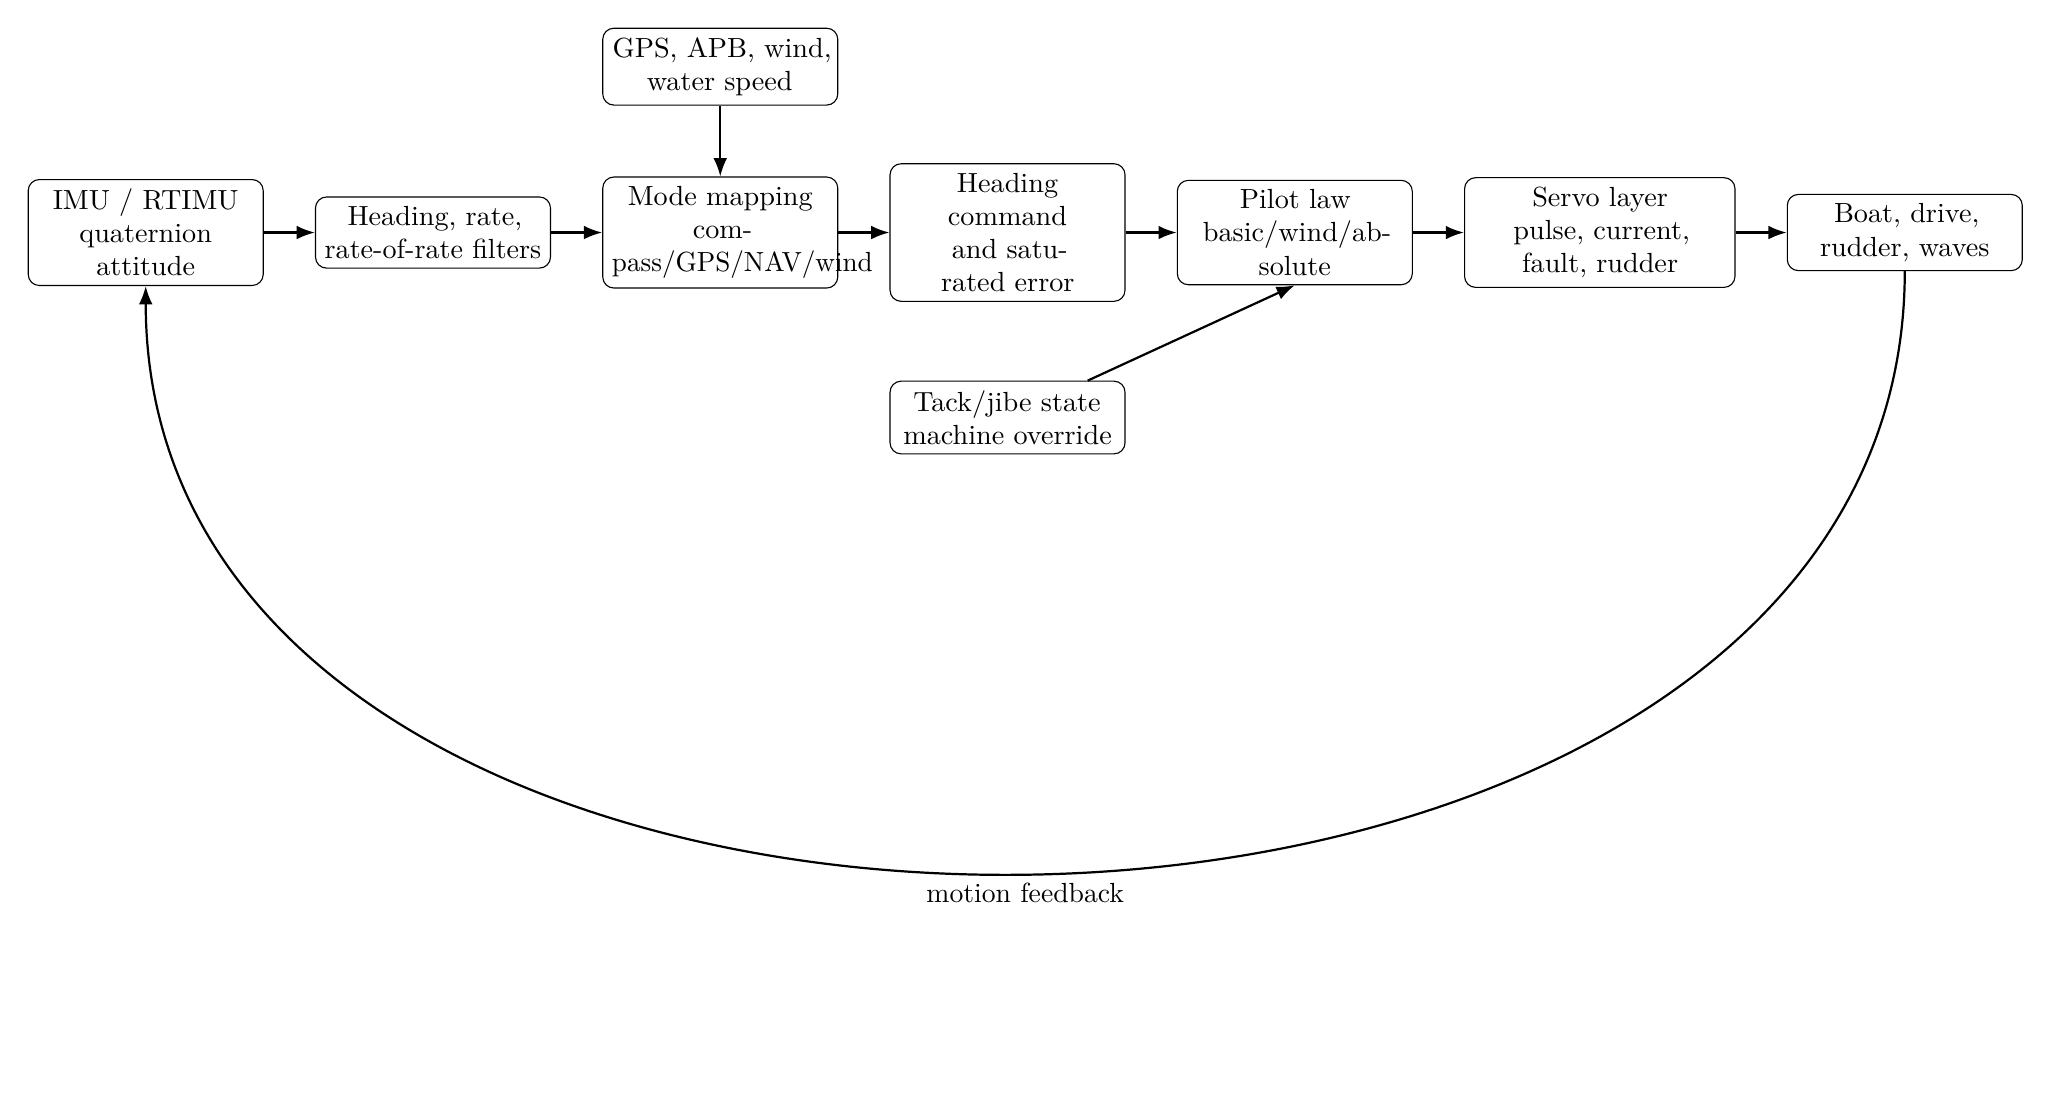
\begin{tikzpicture}[
  node distance=0.45cm and 0.65cm,
  block/.style={draw, rounded corners, align=center, minimum height=0.82cm, text width=2.75cm},
  wide/.style={draw, rounded corners, align=center, minimum height=0.82cm, text width=3.2cm},
  arrow/.style={-Latex, thick}
]
\node[block] (imu) {IMU / RTIMU\\quaternion attitude};
\node[block, right=of imu] (signals) {Heading, rate,\\rate-of-rate filters};
\node[block, right=of signals] (mode) {Mode mapping\\compass/GPS/NAV/wind};
\node[block, right=of mode] (error) {Heading command\\and saturated error};
\node[block, right=of error] (pilot) {Pilot law\\basic/wind/absolute};
\node[wide, right=of pilot] (servo) {Servo layer\\pulse, current, fault, rudder};
\node[block, right=of servo] (boat) {Boat, drive,\\rudder, waves};

\draw[arrow] (imu) -- (signals);
\draw[arrow] (signals) -- (mode);
\draw[arrow] (mode) -- (error);
\draw[arrow] (error) -- (pilot);
\draw[arrow] (pilot) -- (servo);
\draw[arrow] (servo) -- (boat);
\draw[arrow] (boat.south) to[out=-90,in=-90,looseness=1.15] node[below, align=center] {motion feedback} (imu.south);

\node[block, below=1.0cm of error] (tack) {Tack/jibe state\\machine override};
\draw[arrow] (tack) -- (pilot.south);

\node[block, above=0.9cm of mode] (nmea) {GPS, APB, wind,\\water speed};
\draw[arrow] (nmea) -- (mode);
\end{tikzpicture}
\caption{Conceptual \texttt{pypilot} control stack in the uploaded source.}
\label{fig:pypilot-stack}
\end{figure*}

\section{Pilot Loading and Active Algorithms}

Pilot modules are discovered dynamically from \texttt{pypilot/pilots}.  A module is
skipped when it declares \texttt{disabled = True}; otherwise a module-level symbol
\texttt{pilot} is appended to the list of available pilot classes.  In the uploaded tree,
the practical active pilots are \texttt{basic}, \texttt{wind}, and \texttt{absolute}; most
adaptive or experimental pilots are disabled or incomplete.  The default selected pilot
is \texttt{basic}.

\begin{table}[h]
\centering
\caption{Pilot modules and operational status in the inspected archive.}
\label{tab:pilots}
\begin{tabularx}{\columnwidth}{@{}lclX@{}}
\toprule
Pilot & Active & Class & Main idea \\
\midrule
\texttt{basic} & yes & \texttt{BasicPilot} & Extended heading PD with feed-forward. \\
\texttt{wind} & yes & \texttt{WindPilot} & Wind-relative heading plus gust term. \\
\texttt{absolute} & yes & \texttt{AbsolutePilot} & Rudder-position command, requires rudder feedback. \\
\texttt{simple} & no & \texttt{SimplePilot} & Classic PID, disabled. \\
\texttt{rate} & no & \texttt{RatePilot} & Turn-rate target loop, disabled. \\
\texttt{gps} & no & \texttt{GPSPilot} & GPS-heading pilot, disabled. \\
\texttt{deadzone} & no & \texttt{DeadZonePilot} & Deadband experiment, disabled. \\
\texttt{fuzzy} & no & \texttt{FuzzyPilot} & Online lookup-table learning, disabled. \\
\texttt{vmg} & no & \texttt{VMGPilot} & VMG table idea, incomplete and disabled. \\
\texttt{learning} & no & \texttt{LearningPilot} & TFLite predictive idea, disabled. \\
\bottomrule
\end{tabularx}
\end{table}

This distinction matters.  The repository contains sketches of learning and VMG control,
but the real steering path in this archive remains deterministic and comparatively simple.

\section{Heading Representation and Error Calculation}

Let \(\heading\) denote the current controlled heading variable and
\(\heading_{\cmd}\) the commanded value.  Depending on mode, \(\heading\) is not always
magnetic compass heading.  The base pilot maps sensor data into a mode-dependent heading:
\begin{align}
\heading_{\mathrm{compass}} &= \heading_c, \\
\heading_{\mathrm{gps}} &= \wrap(\heading_c + \Delta_{g/c}), \\
\heading_{\mathrm{wind}} &= \wrap(\Delta_{w/c} - \heading_c), \\
\heading_{\mathrm{true\ wind}} &= \wrap(\Delta_{tw/c} - \heading_c),
\end{align}
where \(\Delta_{g/c}\), \(\Delta_{w/c}\), and \(\Delta_{tw/c}\) are slowly updated offsets
between compass, GPS course, apparent wind, and true wind references.

The signed angular wrapping operation is represented by
\begin{equation}
  \wrap(a; b) \in (b-180^{\circ}, b+180^{\circ}],
\end{equation}
matching the source function \texttt{resolv(angle, offset)}.  The heading error is then
clipped:
\begin{equation}
  e = \clip\!\left(\wrap(\heading - \heading_{\cmd}), -30^{\circ}, 30^{\circ}\right).
  \label{eq:error-clip}
\end{equation}
For wind modes the sign is reversed, because apparent wind direction is defined as where
the wind is coming from, not where the vessel is traveling.

This saturation is a practical marine choice.  It prevents the inner controller from
seeing very large error after a sensor jump, tack, gybe, compass recalibration, or command
change.  It also means \texttt{pypilot} prefers bounded correction over aggressively
trying to unwind a large angular error.

\section{The Default Basic Pilot}

The default basic pilot computes heading rate \(\dot{\heading}\) and heading-rate-rate
\(\ddot{\heading}\) from the IMU-derived signals
\texttt{headingrate\_lowpass} and \texttt{headingraterate\_lowpass}.  The active control
law can be written as
\begin{equation}
\begin{split}
  u_b ={}& K_P e
        + K_D \dot{\heading}
        + K_{DD} \ddot{\heading}
        + K_{PR}\,\sgn(e)\sqrt{\abs{e}} \\
        &+ K_{FF}\dot{\heading}_{\cmd} .
\end{split}
\label{eq:basic}
\end{equation}

Here \(u_b\) is the requested servo command before the lower servo layer reshapes it.  The
square-root term is computed explicitly from heading error:
\begin{equation}
  e_{PR} = \sgn(e)\sqrt{\abs{e}}.
  \label{eq:pr}
\end{equation}

The terms in \cref{eq:basic} have intuitive roles:
\begin{itemize}
\item \(K_P e\): proportional correction from course error;
\item \(K_D\dot{\heading}\): gyro counter-rudder or yaw-rate damping;
\item \(K_{DD}\ddot{\heading}\): damping against rapidly changing yaw rate;
\item \(K_{PR}e_{PR}\): nonlinear low-error authority without a purely high linear gain;
\item \(K_{FF}\dot{\heading}_{\cmd}\): feed-forward during commanded course changes.
\end{itemize}

The interesting part is the combination of \(D\), \(DD\), and \(PR\).  A commercial pilot
might expose related concepts as \emph{gain}, \emph{counter rudder}, \emph{response}, or
\emph{sea state}; \texttt{pypilot} exposes the actual additive terms.

\section{Integral Action and Bias Handling}

The main autopilot maintains an integrated heading error,
\begin{equation}
  I_{k+1} = \clip\!\left(I_k + \frac{e_k}{50}\Delta t, -10, 10\right),
  \label{eq:integral}
\end{equation}
but the default basic and wind pilots comment out the \(I\) term.  The code also reduces
or resets this integral around mode changes and command changes.  This is conservative:
it avoids integral windup in waves and maneuvers, but persistent biases such as weather
helm, current, or asymmetric drive behavior are not estimated as an explicit disturbance
state in the active pilot.

A more model-based heading controller would estimate a slowly varying yaw bias,
\begin{equation}
  b_{k+1} = b_k + \eta_k,
\end{equation}
and subtract it from the required control.  In this archive, comparable behavior is
handled indirectly through offsets, manual gain tuning, servo calibration, and the lower
servo windup/pulse mechanism.

\section{Heading-Command Feed-Forward}

When the autopilot is enabled, the main loop computes a filtered heading-command-rate
signal from the difference between the current and previous commands:
\begin{equation}
  \dot{\heading}_{\cmd,k}
  = (1-\alpha)\dot{\heading}_{\cmd,k-1}
    + \alpha\,\wrap(\heading_{\cmd,k}-\heading_{\cmd,k-1}),
  \qquad \alpha \approx 0.1.
\end{equation}
For non-wind modes the sign is reversed before filtering.  This gives the controller a
feed-forward term during user-initiated course changes or tack state transitions.  It is
not a reference-model trajectory generator; it is a first-order filtered command-difference
signal.

\section{Wind Pilot}

The wind pilot preserves the same general heading-control structure, but it changes how
the controlled heading is defined.  In apparent wind mode,
\begin{equation}
  \heading = \AWA,
\end{equation}
while in GPS or compass modes it can synthesize a GPS- or compass-like heading from wind
offsets.  It also computes a wind-gust signal
\begin{equation}
  g_w(k) = V_w(k)-V_w(k-1),
\end{equation}
with a sign adjustment depending on wind direction.  The wind-pilot command is therefore
approximately
\begin{equation}
  u_w = K_P e + K_D\dot{\heading} + K_{DD}\ddot{\heading} + K_{WG}g_w.
  \label{eq:wind}
\end{equation}

This is a useful sailing-specific heuristic, but it is not a full aerodynamic model.  It
does not estimate sail force, rudder lift, polar performance, or wave phase.  It is a
simple, inspectable wind-aware heading controller.

\section{NAV/APB Mode}

The APB sensor handler implements a very compact route-following law.  If an APB sentence
provides route track \(\chi_r\) and cross-track error \(x_{te}\), then the heading command
is
\begin{equation}
  \heading_{\cmd} = \chi_r + K_{xte} x_{te}.
  \label{eq:apb}
\end{equation}
The source default is \(K_{xte}=300\), documented in a comment as roughly
\(30^{\circ}\) for \(0.1\) nautical mile.

This design is much simpler than modern path-following controllers.  It has no explicit
look-ahead distance, no velocity-dependent lateral-acceleration target, no curvature
planning, and no inner yaw-rate target.  The advantage is simplicity and compatibility
with common NMEA/APB navigation data.  The disadvantage is weaker behavior in current,
tight routes, variable speed, and overshoot-prone waypoint transitions.

\section{Tack and Gybe State Machine}

The tack module is a supervisory override.  Its states are
\begin{equation}
  \mathcal{S}=\{\texttt{none},\texttt{begin},\texttt{waiting},\texttt{tacking}\}.
\end{equation}
The tack direction is inferred from wind direction when possible, or from heel if enabled.
During \texttt{tacking}, the normal pilot is bypassed and the servo receives
\begin{equation}
  u_t = \clip\!\left(1 + \frac{\dot{\heading}+\ddot{\heading}/2}{r_t}, -1, 1\right)
\end{equation}
up to a direction sign, where \(r_t\) is the configured tack rate.  Completion is detected
when a normalized progress variable exceeds a configured threshold.  The command heading
is then switched to the new tack heading.

This is intentionally simple: it is a maneuver state machine, not an optimal tack planner.
It does not time the tack using waves or boat speed, and it does not evaluate alternative
tacking strategies.  Adaptive tack-strategy selection is a separate research topic in
robotic sailing literature and is not implemented in the active \texttt{pypilot} code path.

\section{Servo and Motor Command Layer}

The servo layer is one of the most distinctive parts of the project.  A pilot output
\(u\) is not simply sent to a rudder.  The normal command path treats \(u\) as a desired
motor-drive speed-like request, then reshapes it using minimum speed, maximum speed,
periodic pulse behavior, current limits, voltage compensation, overcurrent end-stop
protection, and rudder feedback when available.

Let \(v_c\) be the desired drive speed after pilot gain.  The layer applies
\begin{equation}
  v_c \leftarrow \clip(v_c, -v_{\max}, v_{\max}),
\end{equation}
and a minimum-motion pulse mechanism.  The source maintains a windup-like accumulator
\begin{equation}
  W_{k+1} = W_k + (v_c - v_k)\Delta t,
\end{equation}
and only emits a nonzero command when the accumulated request is large enough to overcome
the configured minimum drive speed over the configured period.  This is a practical answer
to real marine actuators: friction, deadband, clutch delay, slow hydraulic response, and
cheap H-bridge motor control.

When rudder feedback is available, the \texttt{absolute} pilot and servo position command
path can use a rudder-position PID-like loop:
\begin{equation}
  u_r = K_{rp}(r_{\cmd}-r) + K_{ri}\bar e_r + K_{rd}\dot r.
\end{equation}
However, the default \texttt{basic} pilot does not require rudder feedback.

\section{IMU and Heading Estimation}

The IMU layer uses RTIMU quaternion fusion, applies alignment calibration, and computes
Euler roll, pitch, and heading from the aligned quaternion.  Quaternion rotation can be
written as
\begin{equation}
  \vct{v}' = \quat{q}\qmul \vct{v}\qmul \qconj{\quat{q}}.
\end{equation}
The source then derives heading rate from the rotated gyro vector and computes low-pass
signals:
\begin{align}
  \heading_{lp,k} &= \alpha_h \heading_k + (1-\alpha_h)\heading_{lp,k-1}, \\
  \dot{\heading}_{lp,k} &= \alpha_r \dot{\heading}_k
     + (1-\alpha_r)\dot{\heading}_{lp,k-1}, \\
  \ddot{\heading}_{lp,k} &= \alpha_a \ddot{\heading}_k
     + (1-\alpha_a)\ddot{\heading}_{lp,k-1}.
\end{align}
Angular wrap is handled specially for heading low-pass filtering so that filtering across
\(0^{\circ}/360^{\circ}\) does not introduce a false large jump.

The heading estimator is not a full vessel INS.  It is primarily an AHRS with marine
alignment and calibration behavior, feeding the heading-control loop.

\section{Optional GPS--Inertial Filter}

The optional GPS filter estimates position and velocity at a higher output rate by
combining GPS updates with acceleration-derived prediction.  In two dimensions the state
can be written as
\begin{equation}
  \vct{x} = \begin{bmatrix} x & y & v_x & v_y \end{bmatrix}\T .
\end{equation}
The prediction model is the constant-acceleration kinematic model
\begin{equation}
  \vct{x}_{k+1} =
  \begin{bmatrix}
  \mat{I} & \Delta t\mat{I} \\
  \mat{0} & \mat{I}
  \end{bmatrix}\vct{x}_k
  +
  \begin{bmatrix}
  \frac{1}{2}\Delta t^2\mat{I} \\
  \Delta t\mat{I}
  \end{bmatrix}\vct{a}_k.
  \label{eq:gps-predict}
\end{equation}
The GPS update uses a standard linear Kalman correction
\begin{align}
  \vct{y}_k &= \vct{z}_k - \mat{H}\vct{x}_k, \\
  \mat{S}_k &= \mat{H}\mat{P}_k\mat{H}\T + \mat{R}, \\
  \mat{K}_k &= \mat{P}_k\mat{H}\T\mat{S}_k\inv, \\
  \vct{x}_k^+ &= \vct{x}_k^- + \mat{K}_k\vct{y}_k, \\
  \mat{P}_k^+ &= (\mat{I}-\mat{K}_k\mat{H})\mat{P}_k^-.
\end{align}
The implementation also keeps a history so that delayed GPS measurements can be applied
at the approximate measurement time and then fast-forwarded through later inertial
predictions.

This is useful, but it is not the core steering controller.  It mostly improves filtered
speed, track, and position availability.

\section{Comparison with ArduPilot Rover}

ArduPilot Rover separates high-level path following from low-level steering-rate control.
Its older navigation documentation describes the L1 controller as the highest-level
steering controller: it accepts position targets and current speed and outputs a desired
lateral acceleration, which then feeds lower-level controllers \cite{ardupilot-l1}.  Its
steering-rate documentation describes a turn-rate PID controller with feed-forward,
proportional, integral, and derivative gains \cite{ardupilot-rate}.

A compact comparison is
\begin{align}
\texttt{pypilot:} \quad
& \chi_r + K_{xte}x_{te} \longrightarrow \heading_{\cmd}
\longrightarrow u_b, \\
\text{ArduPilot-style:} \quad
& \text{path geometry},\ \SOG
\longrightarrow a_y^{\cmd}
\longrightarrow \dot{\heading}^{\cmd}
\longrightarrow u.
\end{align}

Thus \texttt{pypilot} is heading-hold centered, whereas ArduPilot Rover is path-following
centered in autonomous modes.  The \texttt{pypilot} approach is lighter and easier to tune
on a sailboat with limited sensors, but it is less rigorous for route tracking.

\section{Comparison with PX4}

PX4 fixed-wing control is even more layered.  PX4 documentation describes TECS for
altitude and airspeed control and NPFG for horizontal heading/position control
\cite{px4-fw}.  That architecture is built for aircraft energy and trajectory control,
with separate inner attitude and rate loops.  A direct comparison to \texttt{pypilot} is
therefore imperfect, but the contrast is useful:
\begin{itemize}
\item PX4 treats the vehicle as a dynamic aircraft with explicit position, attitude,
energy, and actuator layers.
\item \texttt{pypilot} treats the sailboat autopilot mainly as a heading servo plus
marine-specific modes and motor protection.
\end{itemize}

The difference is not just sophistication.  The vehicles are different.  A small sailboat
autopilot often needs low power, reliable clutch/motor handling, wind modes, and tolerance
of slow response more than it needs aggressive trajectory tracking.

\section{Comparison with Commercial Marine Pilots}

OpenPlotter documentation presents \texttt{pypilot} as a modular open-source marine
autopilot supporting compass, GPS/NAV, wind, and true-wind modes, with an IMU, optional
GPS/wind sources, motor controller, and drive hardware \cite{openplotter-pypilot}.  B\&G
pilot materials similarly describe wind and navigation modes and manual course adjustments
from pilot controls \cite{bg-pilot}.  B\&G sailing guidance also describes true-wind-angle
use for gybing \cite{bg-setup}.

The practical difference is visibility.  Commercial pilots may provide polished
commissioning, proprietary sea-state adaptation, and integrated displays, but the actual
control laws are hidden.  \texttt{pypilot} exposes the terms, gains, and source code.
That is a major advantage for experimentation, but it also means incomplete experimental
code is visible in the tree.

\section{Experimental and Incomplete Algorithms}

The repository contains several ideas that are not part of the active default control path.

\subsection{VMG Table Pilot}

The VMG pilot attempts to collect measurements of speed and track versus heading on each
tack, storing them in heading-indexed tables.  Conceptually, one would estimate
\begin{equation}
  \mathrm{VMG}(\heading) = \vct{v}(\heading)\cdot \hat{\vct{d}},
\end{equation}
where \(\hat{\vct{d}}\) is the desired progress direction.  The command would then move
toward
\begin{equation}
  \heading^* = \arg\max_{\heading} \mathrm{VMG}(\heading).
\end{equation}
In the uploaded file this optimizer is not implemented; the relevant block contains a
\texttt{pass}.  The module is also disabled.

\subsection{Fuzzy Pilot}

The fuzzy pilot defines a multi-dimensional interpolation table over ground speed, wind
speed, wind direction, rudder angle, heel, sea state, heading error, and heading rate.
It recursively interpolates the table to compute a command and updates old table entries
from a delayed error signal.  The learning update is approximately
\begin{equation}
  c_{new} = \clip(c_{old} + \lambda\epsilon, -1, 1),
\end{equation}
where \(\epsilon\) is a delayed heading/rate error proxy.  This pilot is disabled.

\subsection{Learning Pilot}

The learning pilot sketches a TensorFlow Lite model-predictive idea: feed a history of
sensor values and candidate future actions to a learned model, predict future outputs, and
choose the action sequence with lowest loss,
\begin{equation}
  J = \sum_i
  \left(K_P \hat e_i + K_D\widehat{\dot{\heading}}_i\right)^2
  + K_W u_i^2.
\end{equation}
This is promising in principle, but in the uploaded tree it is disabled and incomplete.

\section{Code-Level Observations}

The following issues are important if these experimental paths are to be revived:
\begin{itemize}
\item \texttt{pilots/vmg.py} contains a misspelling, \texttt{heading\_comand}, where
\texttt{heading\_command} is intended.
\item \texttt{pilots/vmg.py} leaves the core optimum-direction calculation unimplemented.
\item \texttt{pilots/autotune.py} references \texttt{cost} in places where
\texttt{self.cost} appears intended.
\item \texttt{pilots/gps.py} calls \texttt{resolve(...)} although the resolver function
in the uploaded tree is named \texttt{resolv(...)}.
\item The active \texttt{wind.py} true-wind branch references \texttt{ap.true\_wind\_sensor};
this property was not found elsewhere in the inspected source tree.
\end{itemize}

These observations do not invalidate the active \texttt{basic} pilot, but they show that
the repository contains research sketches as well as production code.

\section{Strengths of the Design}

The main strengths are:
\begin{enumerate}
\item \textbf{Explicit control law.}  The default controller is mathematically simple and
visible in the source.
\item \textbf{Excellent practical actuator attention.}  The servo layer handles motor and
rudder realities that many abstract autopilot algorithms ignore.
\item \textbf{Marine-specific heading modes.}  Compass, GPS/NAV, wind, and true-wind
concepts are built into the architecture.
\item \textbf{Low computational burden.}  The core controller is suitable for Raspberry Pi
class hardware and modest update rates.
\item \textbf{Hackability.}  Gains, modes, and experimental pilots can be inspected and
changed without reverse engineering a proprietary pilot.
\end{enumerate}

\section{Weaknesses and Upgrade Direction}

The main weakness is not the basic heading loop; it is the lack of a stronger guidance
layer above it.  NAV mode should be upgraded before any machine-learning approach is
attempted.  A natural deterministic roadmap is:
\begin{enumerate}
\item keep the existing servo protection and calibration layer;
\item keep the AHRS and heading-mode architecture;
\item replace \cref{eq:apb} with an L1, pure-pursuit, or Stanley-style path follower;
\item add a speed-aware yaw-rate target layer;
\item use rudder-angle feedback when available;
\item add a slow weather-helm/current bias estimator;
\item only then revive VMG/polar optimization.
\end{enumerate}

A possible marine guidance layer would compute a desired lateral acceleration
\begin{equation}
  a_y^{\cmd} = f(\text{path}, \vct{p}, \vct{v}, L_1),
\end{equation}
convert it to a desired turn rate
\begin{equation}
  \dot{\heading}^{\cmd} \approx \frac{a_y^{\cmd}}{\max(V, V_{min})},
\end{equation}
and then use a rate loop or extended heading loop to command the existing servo layer.
This keeps the best part of \texttt{pypilot}---its actuator realism---while improving
route tracking.

\section{Conclusion}

The uploaded \texttt{pypilot} source is best characterized as a practical, open, marine
heading autopilot rather than a full modern autonomous-navigation stack.  Its default
method is an extended PD heading controller with gyro damping, yaw-acceleration damping,
square-root heading-error shaping, and heading-command feed-forward.  Its strongest
engineering feature is the servo/motor layer, which treats real rudder drives as nonlinear,
limited, fault-prone devices rather than ideal actuators.

Compared with ArduPilot or PX4, \texttt{pypilot} has a much simpler guidance layer and a
less formal state-estimation/control hierarchy.  Compared with commercial sailing pilots,
it is less polished and contains incomplete experimental code, but it is transparent,
modifiable, and deeply oriented toward real DIY marine drives.  The most valuable next step
is not to replace it with machine learning, but to add a stronger deterministic guidance
layer above the existing heading and servo architecture.

\begin{thebibliography}{9}

\bibitem{ardupilot-l1}
ArduPilot Dev Team,
\emph{Rover: Tuning Navigation}.  Describes Rover navigation tuning and the L1 controller.
\url{https://ardupilot.org/rover/docs/rover-tuning-navigation-420.html}

\bibitem{ardupilot-rate}
ArduPilot Dev Team,
\emph{Rover: Tuning Turn Rate}.  Describes the steering-rate PID controller and FF/P/I/D tuning.
\url{https://ardupilot.org/rover/docs/rover-tuning-steering-rate.html}

\bibitem{px4-fw}
PX4 Autopilot,
\emph{Fixed-wing Altitude/Position Controller Tuning}.  Describes TECS and NPFG in PX4 fixed-wing control.
\url{https://docs.px4.io/main/en/config_fw/position_tuning_guide_fixedwing}

\bibitem{openplotter-pypilot}
OpenPlotter Documentation,
\emph{Pypilot}.  Describes pypilot components and compass, GPS/NAV, wind, and true-wind modes.
\url{https://openplotter.readthedocs.io/latest/pypilot/pypilot_app.html}

\bibitem{bg-pilot}
B\&G Sailing,
\emph{Autopilot Displays/Controllers}.  Describes Wind and Navigation auto-steering modes and pilot controls.
\url{https://www.bandg.com/en-sg/bg/type/autopilots/autopilot-displays-controllers/}

\bibitem{bg-setup}
B\&G Sailing,
\emph{Autopilots: Setting up your Autopilot}.  Discusses true-wind-angle use in shorthanded gybing practice.
\url{https://www.bandg.com/en-sg/blog/autopilots-setting-up-your-autopilot/}

\end{thebibliography}

\end{document}
